%\documentclass[notes=only]{beamer}   % only notes
\documentclass[handout,
	%notes, 
	12pt]{beamer}
%%% The following snipet is from https://tex.stackexchange.com/questions/6348/problem-with-beamers-pause-in-alignments/6352
\mode<presentation> { \setbeamercovered{%transparent
	invisible} }
\setbeamertemplate{navigation symbols}{}
\makeatletter
\def\beamerorig@set@color{%
  \pdfliteral{\current@color}%
  \aftergroup\reset@color
}
\def\beamerorig@reset@color{\pdfliteral{\current@color}}
\makeatother
%%% ... attempt to make pause work in an align environment because I really wanted this effect
\usepackage{lmodern} % this package avoids a pdftex font compile error

\usepackage{xcolor}
%\usepackage{subfiles}
%\usepackage{multicol}
\usepackage{url}
\usepackage{tikz}
%\usepackage{tkz-euclide}
%\usetkzobj{all}
\usepackage{comment}
\usepackage[mathscr]{euscript}
%\usepackage{enumerate}
%\usepackage{paralist}
\usepackage[all,pdf]{xy}
	\CompileMatrices
\usepackage{cancel}	
\usepackage{comment}
\usepackage{multicol}
%\usepackage{enumitem}
%\setenumerate[itemize]{label=\usebeamerfont*{itemize item}%
%  \usebeamercolor[fg]{itemize item}
%  \usebeamertemplate{itemize item}}
	
\usetheme{Warsaw}
\definecolor{GTblue}{RGB}{0,48,87}
\colorlet{powCol}{blue!75!black}
\colorlet{bkCol}{blue}
\usecolortheme[named=powCol]{structure}
\usecolortheme{beaver}
\setbeamercolor{titlelike}{fg=powCol}	
\setbeamercolor{palette primary}{fg=powCol}
\setbeamercolor{palette secondary}{fg=powCol}
\setbeamercolor{palette tertiary}{fg=powCol}
\setbeamercolor{palette quaternary}{fg=powCol}
\setbeamercolor{normal text}{fg=powCol}
\usebeamercolor*{normal text}

% % % % % % % % % % 

\title[``Do-nothing" Congress]{``Do-nothing" Congress}
\subtitle{Will a bill introduced in the \\ 118th U.S. Congress become a law? %\small  \\ 
	%\footnotesize 
	}% \\
	% \\
	%
\author[A. K. W. Warren]{
    Ashley K. W. Warren
	%\vspace{-0.75pc}
	}
%\institute{\color{GTblue}Georgia Tech%
%	%\vspace{-0.6pc}
%	}
\date{%\small 
	1 June 2024}
\logo{background from \emph{The Picture Show: Photo Stories from NPR} by Kent Nishimura/Los Angeles Times}

% % % % % 
\begin{document}

\usebackgroundtemplate{
	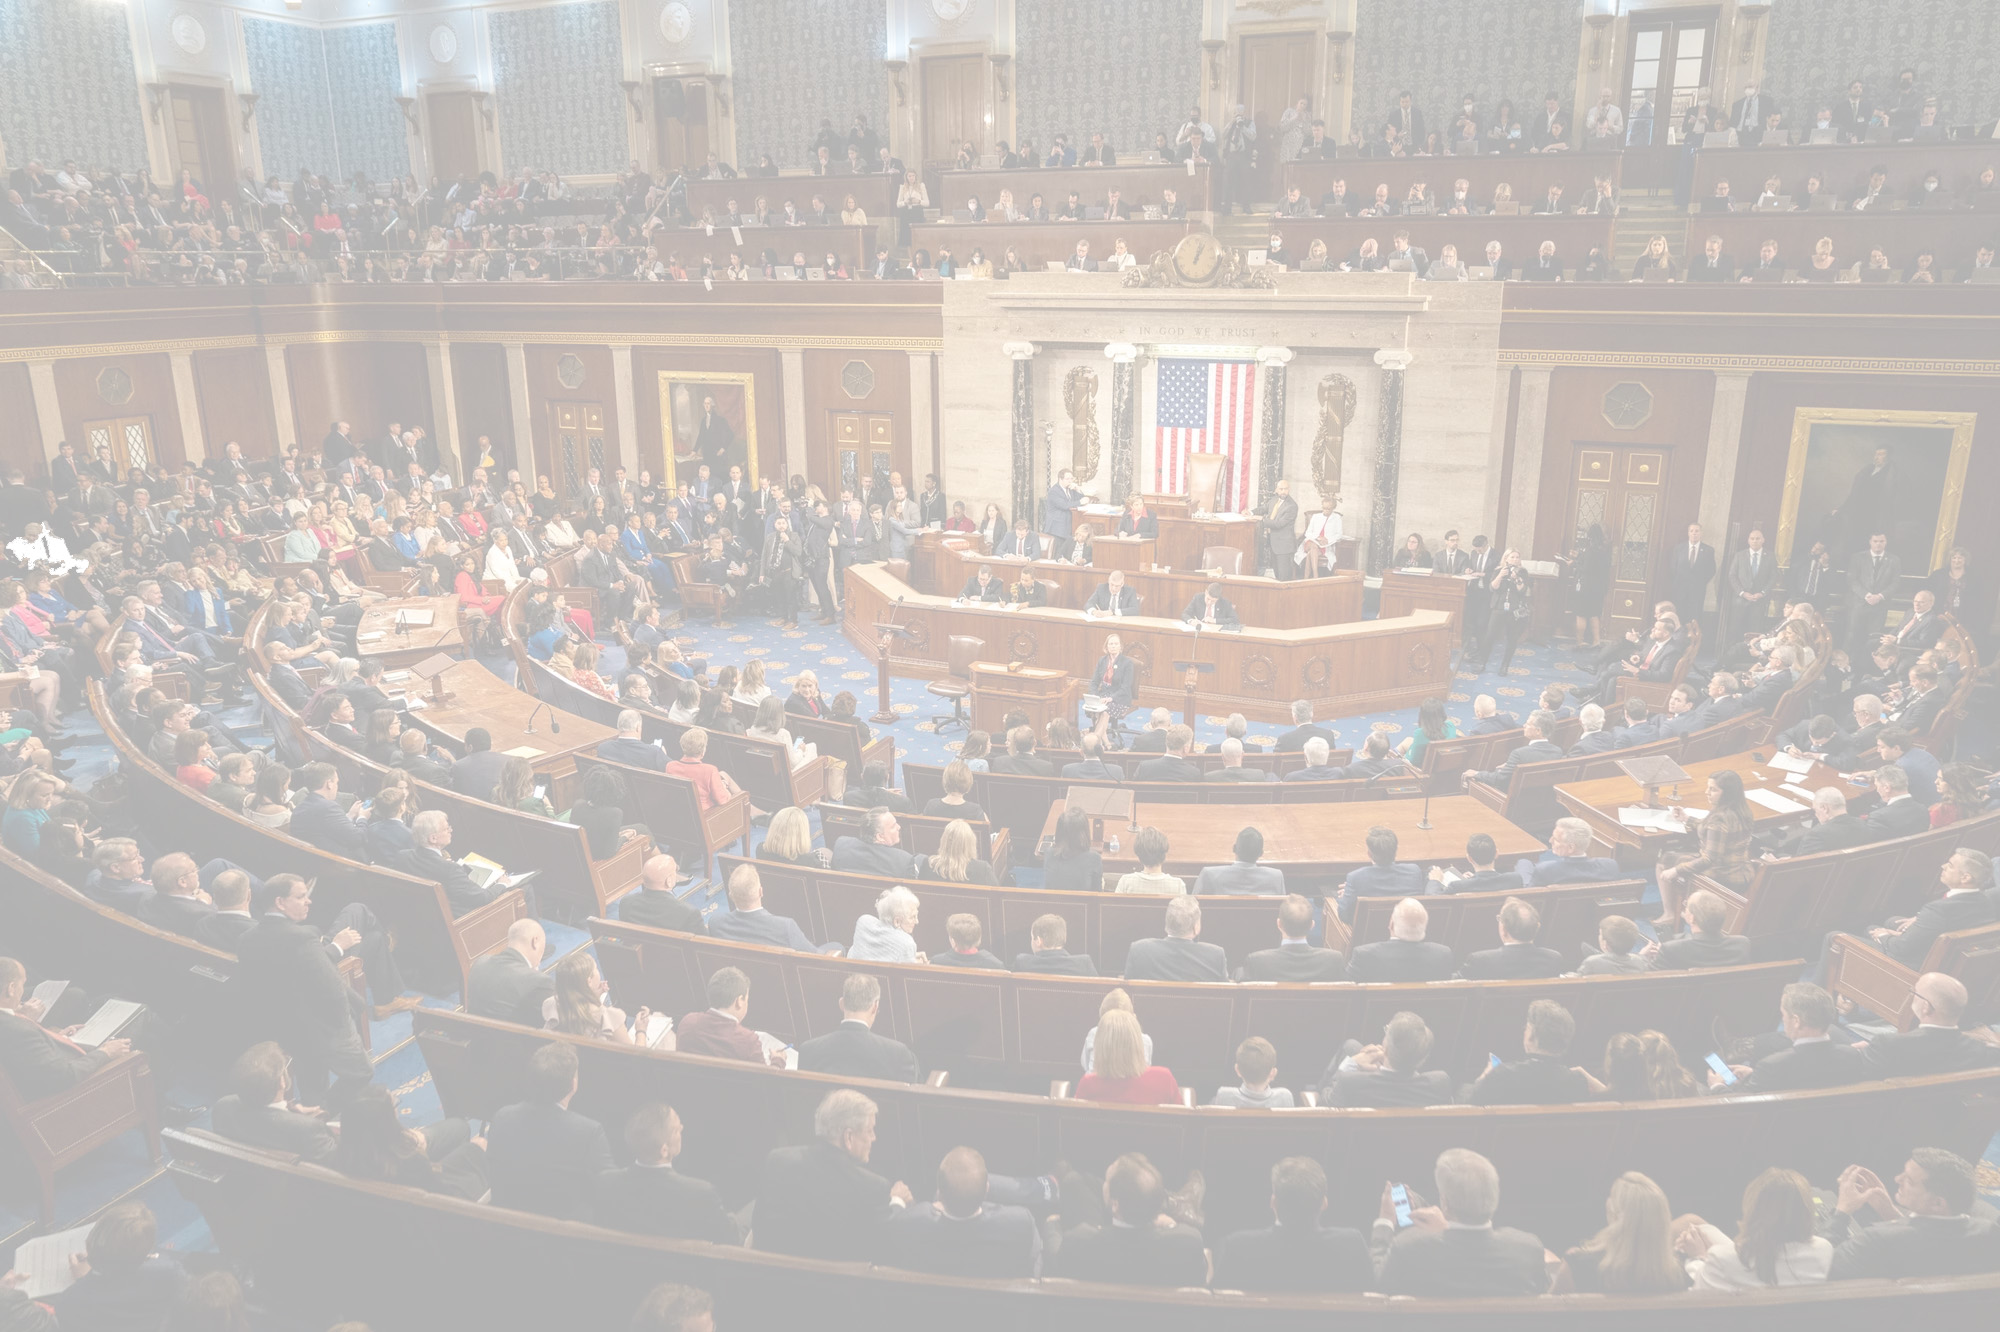
\includegraphics[width=\paperwidth,height=\paperheight]{118presentationfiles/housefirstday.jpg}
	}
	
% % %
\begin{frame}
%\large
\titlepage
\end{frame}

\usebackgroundtemplate{
	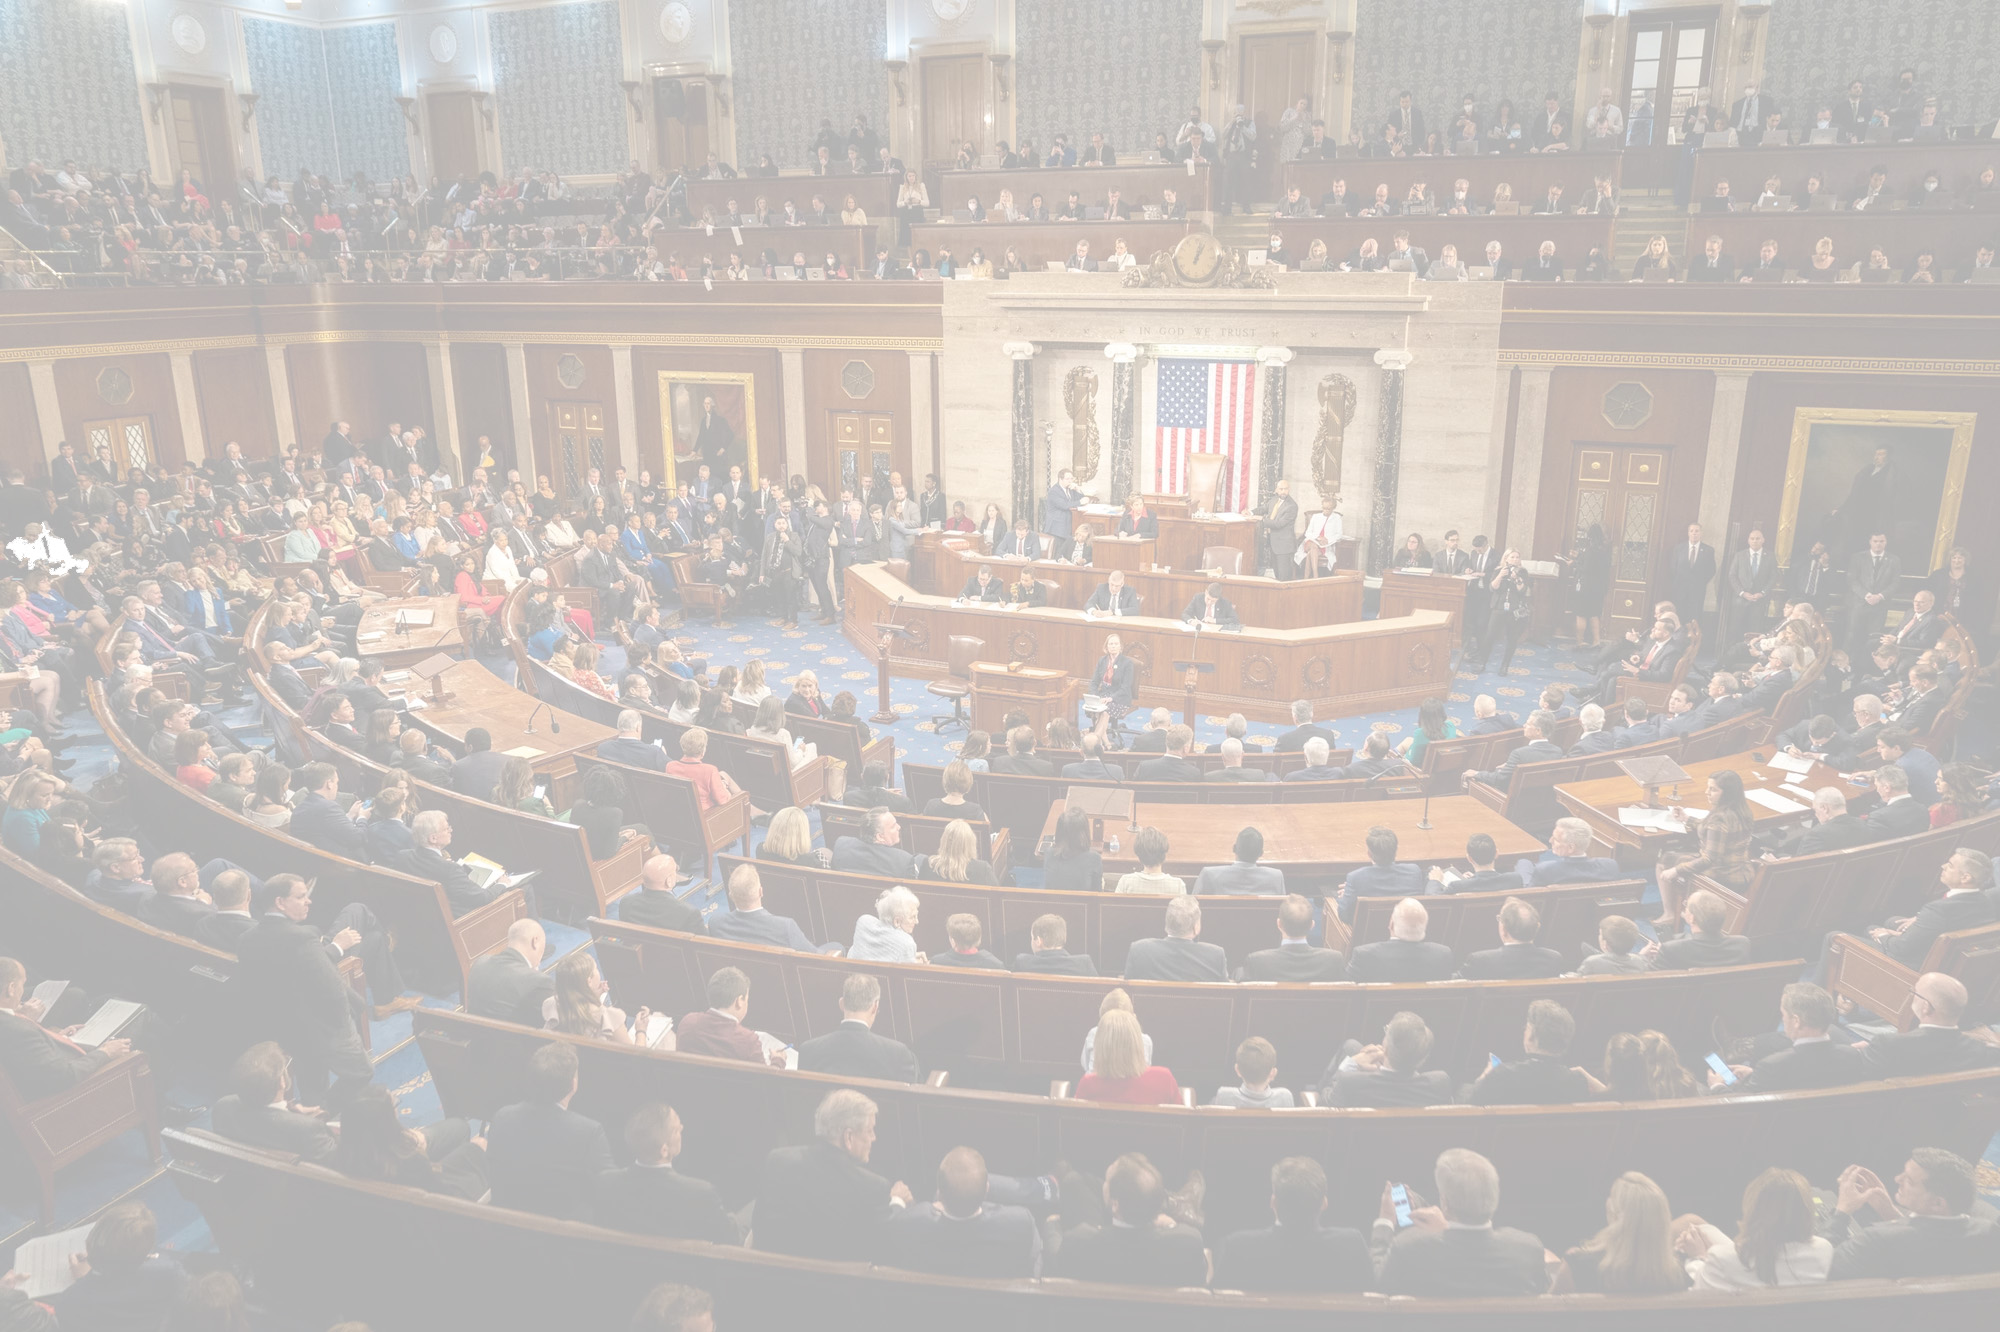
\includegraphics[width=\paperwidth,height=\paperheight]{118presentationfiles/housefirstday.jpg}
	}

% % %
\begin{frame}{Data}{}
\pause
\begin{itemize}
\item Legiscan API: https://legiscan.com/datasets
\pause
\item Over 15,000 bills introduced in the 118th Congress.  As of 1 June 2024, only 64 have become law!
\pause
\item For each bill, initial\_data\_cleaning.json stores:

\vspace{-0.5pc}
\begin{multicols}{2}
{\small
\begin{itemize}
\itemsep0em
\item chamber in which the bill was introduced
\item type (bill, resolution, joint resolution, concurrent resolution)
\item bill's title
\item a summary of the bill
\item date the bill was introduced
\end{itemize}
}
\end{multicols}
\end{itemize}
\end{frame}
	
% % % %
\note{
\begin{itemize}
\end{itemize}
}

% % % 
\begin{frame}{Data, cont.}
\begin{itemize}
\item[]
\begin{multicols}{2}
{\small
\begin{itemize}
\itemsep0em
\item sponsor(s): 
{\footnotesize 
\begin{itemize}
\itemsep0em
\item people with name, party, and state
\item number of sponsors from each party
\end{itemize}
}
\item subject(s)
\item number of actions
\item latest action
\item whether it passed in the House, and if so, date and votes:
{\footnotesize
\begin{itemize}
\itemsep0em
\item people: name, party, state, vote (yea, nay, absent, not voting)
\item number of each type of vote from each party
\end{itemize}
}
\item same information about whether it passed in the Senate
\item whether it became law, and if so, the date
\end{itemize}
}
\end{multicols}
\end{itemize}
\end{frame}

% % %
\begin{frame}{Four data sets}{}
The problem is a classification problem between two classes (will the bill become law or not?), so we went with logistic regression.  

\pause
\vspace{1pc}
\underline{Issue}:  Imbalanced data.  Out of 15,366 bills only 64 became law.  This means an algorithm that predicts a bill will never become law is technically accurate 99.6\% of the time!  We need a model that can out-perform that.
\end{frame}

% % % 
\begin{frame}{Four data sets, cont.}{}
To address the imbalance, we created 4 data sets to train:

\pause
\begin{multicols}{2}
\begin{itemize}
\itemsep0em
\item all bills (15,366)
\pause
\item bills that passed in the House (539)
\pause
\item bills that passed in the Senate (189)
\pause
\item bills that passed in both chambers (81)
\end{itemize}
\end{multicols}
\pause
As the accuracy of the baseline model decreases with each data set, we also measure precision and recall.
\end{frame}

% % % 
\begin{frame}{Feature selection}{}
To simplify the model, we reduced to the following features:
\pause
\begin{itemize}
\itemsep0em
\item chamber
\item bill type
\item subject(s)
\item sponsor(s)
\item number of actions
\item a subset of House votes by politician and the numbers by party
\item a subset of Senate votes by politician and the numbers by party
\end{itemize}
\pause
%The subsets of votes by politician differed, depending on the data set, as different correlations showed up in the analysis.
\end{frame}

% % %
\begin{frame}{Results}{}
Which model performed the best?  

\pause
\vspace{1pc}
Overall, the model which only trained on the bills that passed in the House performed the best.  Here's how it did on the test data:

\pause
\begin{itemize}
%\itemsep0em
\item accuracy: 94.3\% \pause (baseline accuracy: 90.7\%)
\pause
\item precision: 80\%
\pause
\item recall: 57.1\%
\end{itemize}
\end{frame}
	
% % %
\begin{frame}{Improvements}{}
One way to improve the model would be to get more information on what specific characteristics, if any, of a bill lead to it becoming a law.  \pause Some ideas:
\pause
{\small
\begin{itemize}
\itemsep0em
\item More dimension reduction.  In the interest of time, didn't really go that in-depth with it and that should be the first place to start.
\pause
\item Use NLP on the titles, summaries, and latest actions on the bills to create tags, then see if specific tags make a bill more likely to become law.  The TagsTest Jupyter notebook has the beginnings of some code from the nltk module.
\pause
\item Parse the dates that events surrounding the bills occurred, then see if the amount of time it takes for an event to occur after the bill's introduction helps determine whether the bill will become law.
\end{itemize}
}
\end{frame}

\usebackgroundtemplate{
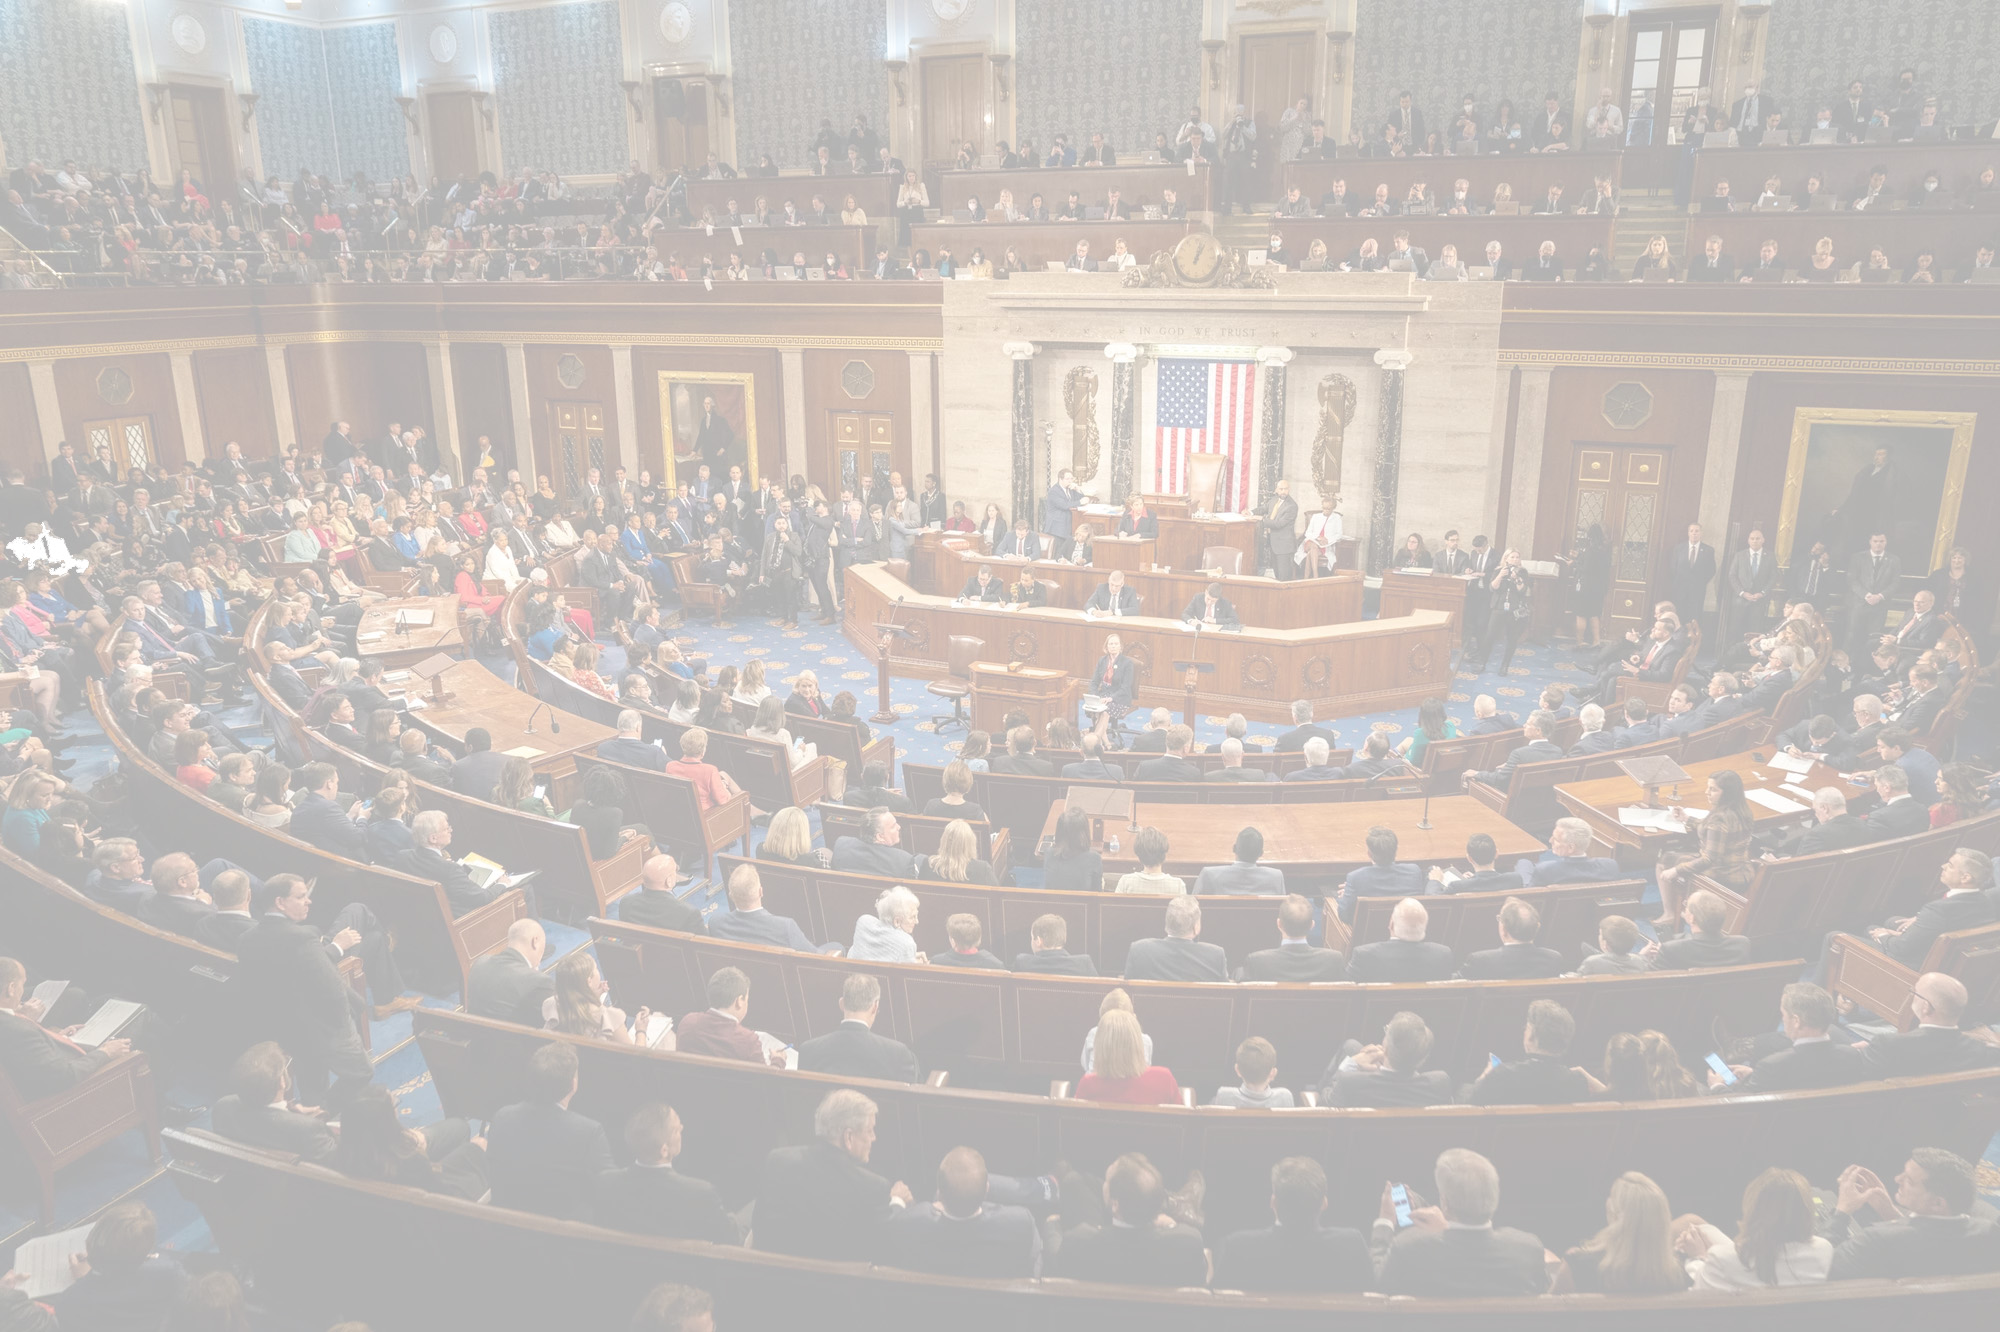
\includegraphics[width=\paperwidth,height=\paperheight]{118presentationfiles/housefirstday.png}
}
	
% % %
\begin{frame}{}{}
\vspace{17pc}
\begin{flushright}
\hspace{50pt}
{\color{gray}U. S. House of Representatives on 3 Jan 2023}
\end{flushright}
\end{frame}

% % % % % % % % % % 
\end{document}